\section{Introduction}

La pyrite, de formule chimique \ce{FeS2}, est plus connue sous le nom de «~pierre à feu~». Elle doit d'ailleurs son nom à sa capacité à produire des étincelles lorsqu'on la frotte ou qu'on la soumet à des chocs avec certains autres matériaux. Longtemps surnommée «~l'or des fous~» de par sa teinte et son aspect qui ont sûrement trompé plus d'un chercheur d'or, la pyrite est aujourd'hui particulièrement utilisée en joaillerie ou dans l'industrie chimique, pour la fabrication d'acide sulfurique. \fxnote{Citation needed}\\
On la trouve naturellement en quantités relativement abondantes dans des gisements à des endroits très divers, en Europe comme en Amérique (lieu d'une «~ruée vers l'or~» au XIXe siècle). Bien qu'elle soit souvent mélangée, par exemple à d'autres composés proches où le fer est substitué par d'autres métaux, il est également possible d'extraire des monocristaux de \ce{FeS2} de taille assez importante sous forme de cubes aux faces lisses ou sous forme de pentagono-dodécaèdres.

\begin{figure}
\caption{Photos d'échantillons cubique et dodécaédrique de cristaux de pyrite.}
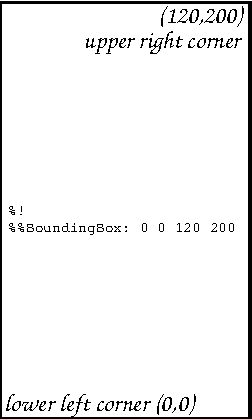
\includegraphics{figures/fig1}
\end{figure}

La pyrite fait donc partie des minéraux que l'on connaît et que l'on a utilisé depuis assez longtemps pour ses propriétés macroscopiques, avant-même de comprendre ses propriétés mésoscopiques et \textit{a fortiori} nanoscopiques.
En réalité, ce cristal a été un des premiers objets d'études de la cristallographie moderne au XXème siècle.\\
Dans cet article, on s'attachera à redéterminer par des expériences de diffraction de rayons X, la structure cristallographique complète de la pyrite, en partant d'une étude macroscopique et jusqu'à retrouver son groupe d'espace et ses paramètres de maille.
% But de l'article : déterminer la structure cristallographique complète de la pyrite

\section{Analyse préalable des symétries cristallines}
% Étude préliminaire : Forme des monocristaux
% Éléments de symétrie et groupe ponctuel du cube
% Éléments de symétrie et groupe ponctuel du pentagono-dodécaèdre

Une étude préalable des symétries des cristaux de pyrite (\ce{FeS2}) sous ses deux principaux faciès cubique et pentagono-dodécaédrique peut permettre de guider le reste de l'étude de ce composé et les expériences (et éventuellement de comprendre l'existence de ces deux conformations).\\
Le cube est le système cristallin ayant le plus d'éléments de symétrie. Il possède~:
\begin{itemize}
    \item 3 axes de rotation d'ordre 4, parallèles aux directions \hmn{<001>} et 3 miroirs orthogonaux à ces axes,
    \item 4 axes de roto-inversion\fxnote{Vérifier} d'ordre 3, le long des diagonales \hmn{<111>},
    \item 6 axes de rotation d'ordre 2, parallèles aux diagonales des faces de directions \hmn{<011>} et 6 miroirs orthogonaux à ces axes,
    \item l'élément de centrosymétrie.
\end{itemize}
Cette combinaison d'éléments de symétrie peut s'écrire en notation d'Hermann-Mauguin sous la forme~:
\[
\hmn{*4 -3 *2}
\]
ou sous la forme condensée \hmn{m-3m}.

% \begin{figure*}[!bt]
%   \centering
%   \subfloat[Dummy sub\label{subfig-1:dummy}]{%
%     \rule{4cm}{3cm}
%   }
%   \subfloat[Dummy sub\label{subfig-2:dummy}]{%
%     \rule{4cm}{3cm}
%   }
%   \caption{Dummy figure with subfigures}\label{fig:dummy}
% \end{figure*}
En observant les éléments de symétrie du pentagono-dodécaèdre, on arrive à en retrouver certains en commun avec le cube, dont on se sert comme base pour désigner les directions des axes. La forme spécifique de pentagono-dodécaèdre prise par la pyrite (pyritoèdre) - que l'on sait différente du dodécaèdre régulier pour éviter tout axe de rotation d'ordre 5, incompatible avec la définition classique d'un cristal - comporte donc les symétries suivantes~:
\begin{itemize}
    \item 3 axes de rotation d'ordre 2 selon les directions \hmn{<001>} et 3 miroirs qui leurs sont orthogonaux,
    \item 4 axes de rotation d'ordre 3 selon les directions \hmn{<111>},
    \item l'élément de centrosymétrie.
\end{itemize}
On s'aperçoit alors que l'objet géométrique ainsi obtenu, qui conserve la majeure partie des éléments de symétrie du cube, appartient bien au système cristallin cubique.
La combinaison de ces éléments se note 
\[
\hmn{*2 -3}
\]
ou de manière plus compacte~: \hmn{m-3}.

À l'échelle macroscopique, la pyrite peut prendre les deux formes géométriques présentées ci-dessus. On suppose que cela vient du fait qu'au cours de la croissance, l'assemblage d'objets du système cristallin cubique, même de symétrie légérement inférieure, est favorisé dans les directions permettant de conserver cette symétrie.\\
Autrement dit, le minéral peut croître en gardant simplement ses symétries propres ou en satisfaisant en plus aux contraintes d'une symétrie d'ordre supérieur.\\
Par cette étude macroscopique, on retiendra alors qu'\textit{a priori} le cristal étudié appartient au système cristallin (et réticulaire) cubique et que son groupe ponctuel est celui possédant les éléments de symétrie du pentagono-dodécaèdre, c'est-à-dire \hmn{m-3}.

\section{Méthodes expérimentales}
% Méthodes expérimentales DRX (Laue + SOLEIL/CRISTAL)

\subsection{Diffraction sur monocristal : méthode de Laue}

Une première expérience de diffraction de rayons X a été réalisée sur des dispositifs spécifiques présents au laboratoire IMPMC de Sorbonne Université, en utilisant la méthode de Laue en transmission (longueur d'onde polychromatique dans un certain intervalle, échantillon fixe pendant la mesure).

La source de rayons X utilisée était un tube à anticathode en cuivre dont la raie \(K_{\alpha_1,\ce{Cu}}\) est de longueur d'onde \(\lambda_{K_{\alpha_1,\ce{Cu}}}=\SI{0.1545}{\nano\metre}\). La cathode en tungstène était excitée avec une tension de \SI{40}{\kilo\volt} (ce qui donne une longueur d'onde minimale \(\lambda_{min} \approx \SI{0.031}{\nano\metre}\)) et un courant de \SI{30}{\milli\ampere}. La lecture du cliché de diffraction de Laue a été réalisée à partir de films réutilisables photosensibles aux RX et numérisés après exposition avec un scanner du même constructeur.\fxnote{Trouver constructeur}

L'échantillon \textit{a priori} monocristallin, placé (après la source) à une distance de \(D = \SI{39}{\milli\metre}\) du détecteur, était monté sur un support permettant un pivot autour de l'axe \hmn{[hkl]}\fxnote{Indiquer direction correcte}.\\
Pour pouvoir observer un diagramme de diffraction et en déduire les éléments de symétrie du cristal puis la classe de Laue, il est nécessaire de l'orienter pour chaque cliché de manière à ce que le faisceau soit parallèle à un ou plusieurs axes et éléments de symétrie.\\
Ici, on a positionné le cristal sous sa forme pyritoédrique manuellement et simplement par appréciation visuelle au travers d'une loupe. Ceci, de manière à ce que le faisceau incident arrive sur le cristal perpendiculairement à une arête verticale, dans l'axe d'une symétrie de type miroir.\\

\subsection{Diffraction par méthode des poudres}

Une mesure de diffraction sur synchrotron a également été réalisée sur la ligne CRISTAL du synchrotron SOLEIL.\fxnote{Citer la ligne CRISTAL} La mesure a été effectuée sur un échantillon poudreux de pyrite (\ce{FeS2}) avec un diffractomètre 2 cercles et pour une longueur d'onde incidente monochromatique correspondant à une énergie \(E_{i,s} = \SI{17017}{\electronvolt}\), soit \(\lambda_{i,s} = \SI{0.07285}{\nano\metre}\).
% Le diffractogramme expérimental obtenu sur la \figref{fig:diffractogrammeSOLEIL} est analysé en \secref{sec:}

\section{Analyse des clichés de Laue}
% Observation des éléments de symétrie du cliché de Laue
% Détermination du groupe de Laue -> comparaison avec le groupe ponctuel supposé et limites des clichés de Laue
% => Diffractogramme sur synchrotron (justifications)

On a vu que les cristaux de pyrite \ce{FeS2} adoptaient une forme cubique ou pentagono-dodécaédrique et on en a déduit que le système réticulaire était le système cubique. \\
L'analyse des clichés de Laue doit permettre, à partir de cette hypothèse, de retrouver le groupe ponctuel identifié précédemment.

\begin{figure}
\caption{Cliché de Laue obtenu par DRX sur un cristal de pyrite orienté de telle manière que le faisceau incident soit orthogonal aux plans \hmn{(hkl)}. On repère assez facilement l'axe de rotation d'ordre 2 et deux miroirs orthogonaux entre eux et contenant l'axe.}
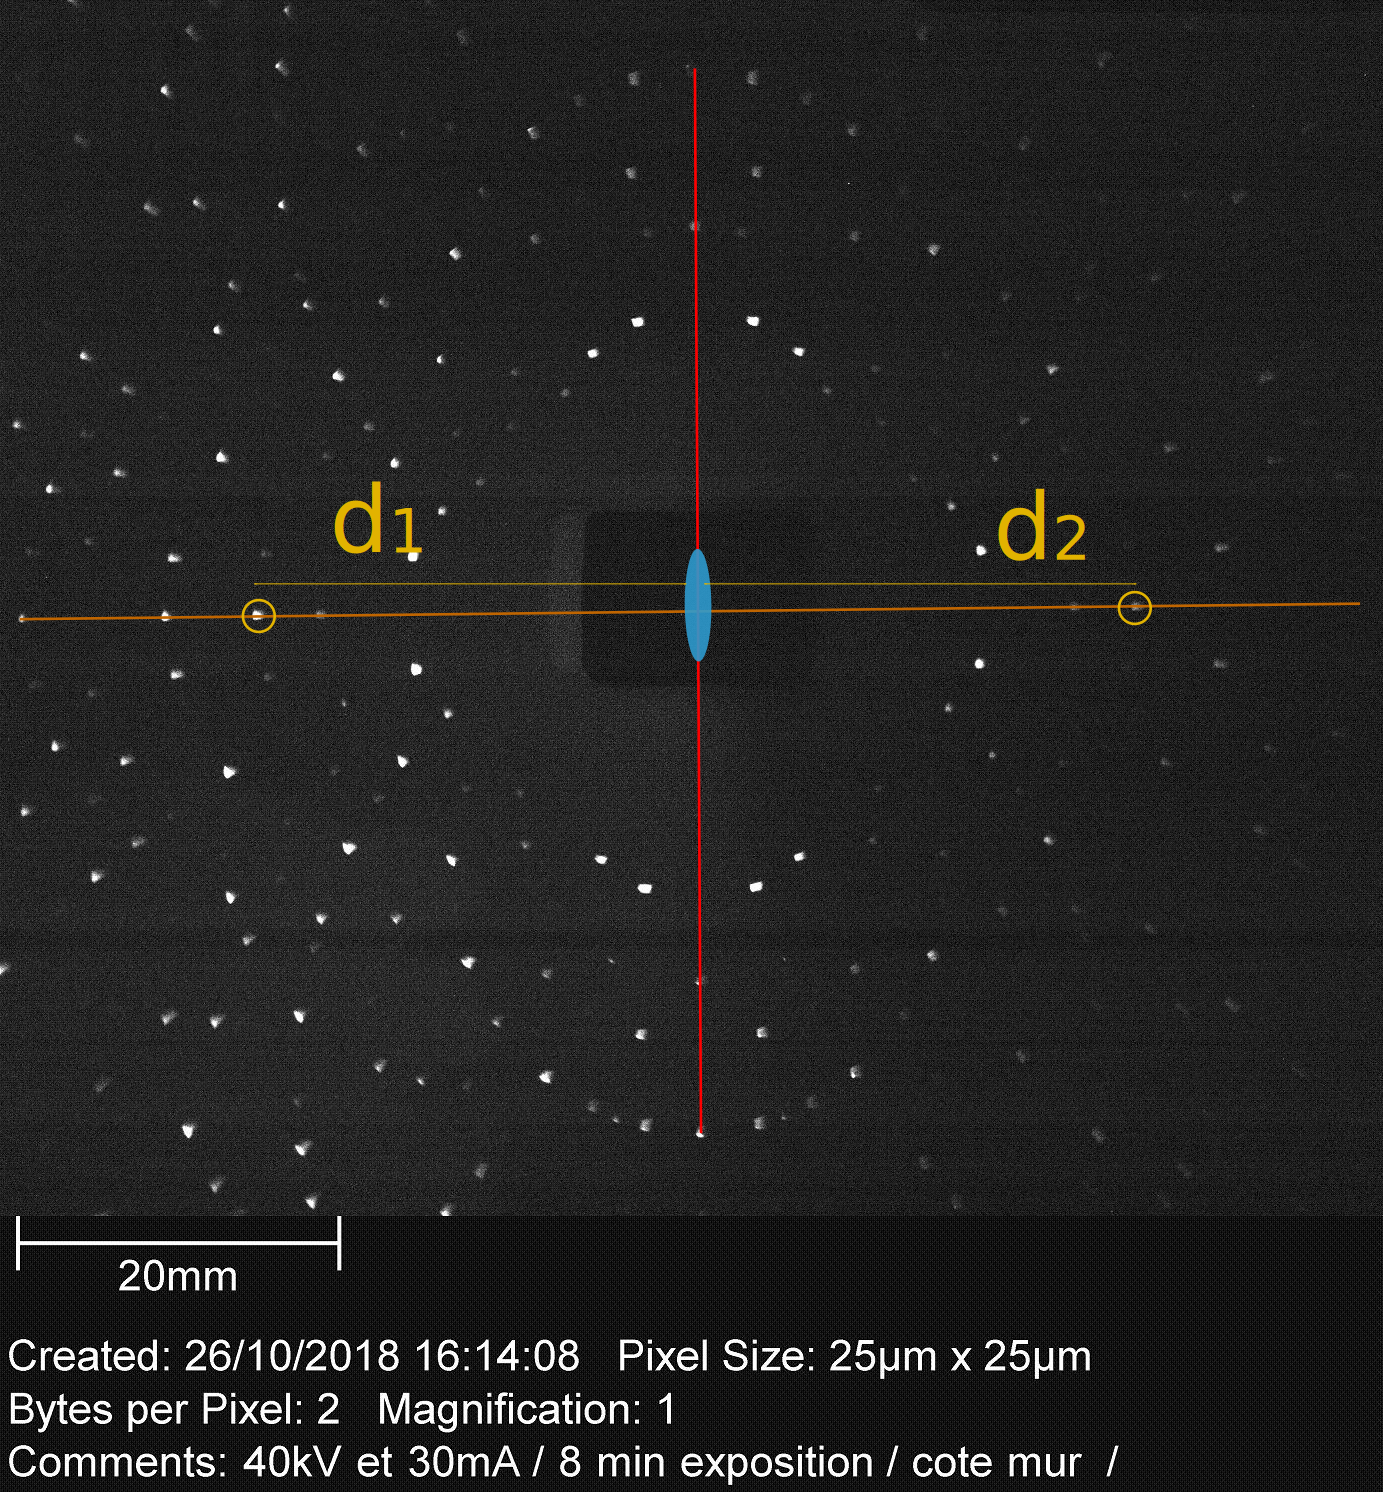
\includegraphics[width=0.85\columnwidth]{figures/Laue_Pyrite_3_symetries}
\label{fig:laueCliche}
\end{figure}

\subsection{Alignement angulaire du cristal}

On s'intéresse à la précision de l'alignement du cristal avec l'axe du faisceau X incident, réalisé par ajustement manuel et à l'œil, au travers d'une loupe.
On calcule une erreur angulaire d'orientation \(\varepsilon\) à partir du cliché de Laue obtenu en \figref{fig:laueCliche} par la formule~:
\begin{equation}
\varepsilon = \frac{1}{4} \left| \arctan\left( \frac{d_1}{D} \right) - \arctan\left(\frac{d_2}{D}\right) \right|,
\end{equation}
où \(D\) est la distance entre l'échantillon et l'écran, \(d_1\) et \(d_2\) sont les distances entre le centre de l'image et deux tâches de part et d'autre de l'image devant être symétriques l'une par rapport à l'autre.\\
Les résultats de cette méthode sont résumés dans la \tableref{tab:LaueAngleError}.
On obtient ainsi un écart de \SI{0.0137}{\degree}, étonamment très faible étant donné les conditions dans lesquelles l'orientation du cristal a été faite.\\
Au vu de cette erreur très faible, le faisceau doit donc arriver avec une assez grande précision le long d'un axe de haute symétrie du cristal, perpendiculairement à la famille de plans \hmn{(hkl)}. Par conséquent, la symétrie du cliché de Laue devrait être quasi-parfaite.

\begin{table}
\caption{Mesures d'écart par rapport à la symétrie attendue et calcul de l'erreur d'alignement angulaire du cristal par rapport à l'axe de haute symétrie proche.}
\label{tab:LaueAngleError}
\begin{tabular}
  {
    >{$}l<{$}
    S[table-format = 2.3(1)]
  }      % Alignment for each cell: l=left, c=center, r=right
% \midrule
 d_1 / \si{\milli\metre}    & 27,494 \\
 d_2 / \si{\milli\metre}    & 27,438 \\
 D / \si{\milli\metre}      & 39 \\
 \varepsilon / \si{\degree} & 0,0137 \\
% \bottomrule
\end{tabular}
\end{table}

\subsection{Symétries, classe de Laue et groupe ponctuel}

Sur la figure de diffraction obtenue en \figref{fig:laueCliche}, on relève un axe de rotation d'ordre 2 et deux miroirs orthogonaux entre eux qui contiennent cet axe.
Il est important de noter qu'il ne s'agit pas d'un axe de rotation d'ordre 4, mais bien d'ordre 2, du fait de la présence/absence de certaines tâches lorsque l'on applique des rotations de \SI{\pi/2}{\radian} (axe d'ordre \hmn{4}) au lieu de \SI{\pi}{\radian} (axe d'ordre \hmn{2}).

La configuration de l'expérience avec le faisceau incident parallèle à un des axes de rotation d'ordre 2 du cristal et deux miroirs orthogonaux, est telle qu'il est normal que l'on ne voit pas d'axes de rotation d'ordre 3 et que l'on retrouve les éléments de symétrie macroscopiques\cite{JJRousseau2007}.\\
Notons que pour retrouver tous les axes de symétrie du cristal et déterminer la classe de Laue sans hypothèse préalable, il aurait fallu faire plusieurs clichés en tournant l'échantillon dans différentes directions.

En regardant les tables de correspondance entre systèmes réticulaires, classes de Laue et groupes ponctuels\cite{JJRousseau2007,ShmueliIUCr2016}, on voit que le système cubique n'offre que deux classes de Laue possibles~: \hmn{m-3} ou \hmn{m-3m}.
La seconde imposant la présence d'un axe de rotation d'ordre 4 est, de fait, incompatible avec le cliché obtenu.\\
Dans le cadre d'une diffusion élastique, les clichés de Laue sont nécessairement centrosymétriques d'après la loi de Friedel \cite{}\fxnote{Citation needed.}, et on ne peut donc pas savoir l'on a affaire à groupe ponctuel centrosymétrique ou non. Dans notre cas, ceci laisse deux groupes ponctuels possibles, associés à la classe de Laue \hmn{m-3}~: \hmn{23} ou \hmn{m-3}.\fxnote{Fix hmn spacing.}

Pour déterminer lequel de ces groupes ponctuels est celui de la pyrite (\ce{FeS2}), il faudrait mener d'autres mesures physiques mais on se contentera ici de se référer à nouveau aux symmétries du cristal repérées précédemment.
Puisque ce cristal comporte un centre d'inversion et des miroirs, on retrouve bien le groupe ponctuel pré-supposé~: \hmn{m-3}.

\subsection{Limites de la méthode de Laue}

Le faisceau de rayons X incident s'étalant sur une certaine plage de longueurs d'onde, il n'est pas techniquement possible de retrouver des paramètres de maille à partir d'un cliché de Laue.\\
La méthode de Laue permet donc d'identifier les directions équivalentes, de retrouver les symétries d'un cristal et sa classe de Laue et peut donc servir à orienter un cristal connu selon un certaine direction pour une autre expérience.
Mais elle ne permet pas de déterminer une structure cristallographique complète.

Pour aller plus loin dans la détermination de la structure de la pyrite, on se propose d'utiliser une autre technique, de diffraction de poudre (méthode de Debye-Scherrer), avec un diffractomètre automatique sur synchrotron.\\
De manière générale, la diffraction de poudre doit permettre, à partir des informations de position angulaire et d'intensité des pics de diffraction, de remonter assez facilement jusqu'au mode de réseau, au groupe d'espace, aux paramètres de mailles et aux positions atomiques dans la maille.
On se permet ici de réduire en poudre l'échantillon plutôt que d'utiliser la méthode du cristal tournant sur un monocristal dans la mesure où la pyrite est relativement abondante et qu'il est facile de se procurer des monocristaux naturels.\\
Par ailleurs, les expériences sur synchrotron permettent d'avoir un grand flux de photons et une meilleure résolution angulaire (utile pour des échantillons multiphases ou composites) et de sélectionner une longueur d'onde précise et donc un faisceau bien monochromatique.\\
On peut ainsi s'affranchir de divers problèmes liés aux équipements de laboratoire comme les forts signaux de fond, les dédoublements de pics dûs aux raies \(K_{\alpha,1}\) et \(K_{\alpha,2}\) et la nécessité d'adapter la source de rayons X (tube de Coolidge et filtre de sélection de raies) en fonction des échantillons observés.
En particulier, on relève que dans le cas présent pour l'échantillon de pyrite (\ce{FeS2}), la pertinence de l'utilisation d'une source de cuivre \ce{Cu} est discutable du fait de la présence d'un seuil d'absorption du fer proche des raies \(K_{\alpha,\ce{Cu}}\) causant un phénomène de fluorescence du fer de l'échantillon.
Pour ce type d'échantillon, une source à anticathode en cobalt \ce{Co} pourrait par exemple être utilisée à la place.

\section{Obtention du mode de réseau}
% Plot données diffractogramme (gnuplot ? matplotlib ? octave ?)
% Tableau des 10 premières raies :  numéro pic, angles 2*theta, d_hkl, d_i+1/d_i, numéro des raies (h²+k²+l²), indices (hkl), paramètre de maille calculé
% Lecture des positions angulaires (2*theta) des 10 premières raies
% Calcul des distances inter-réticulaires (Loi de Bragg)
% Calcul des valeurs de rapport entre distances inter-réticulaires (di+1/di)
% Intérêt de ces rapports et comparaison des valeurs expérimentales avec des rapports calculés
% Obtention des indices hkl pour chacune des raies et détermination du mode de réseau (primitif, sinon il y aurait plus d'extinctions -> facteur de structure décomposé en mode+motif)

Le diffractogramme obtenu sur synchrotron est donné sur la \figref{fig:soleilPowderDiffractogram} et l'ensemble des valeurs relevées et calculées à partir de cette figure sont indiquées dans le \tableref{tab:peaksParameters}.

\begin{figure}
\caption{Diffractogramme de l'échantillon de poudre de pyrite (méthode de Debye-Scherrer) mesuré sur la ligne CRISTAL du synchrotron SOLEIL, pour une longueur d'onde \(\lambda_{i,s} = \SI{0.07285}{\nano\metre}\). Les intensités sont «normalisées» (divisées de manière à ce que l'intensité du pic de plus haute intensité atteigne la valeur 100).}
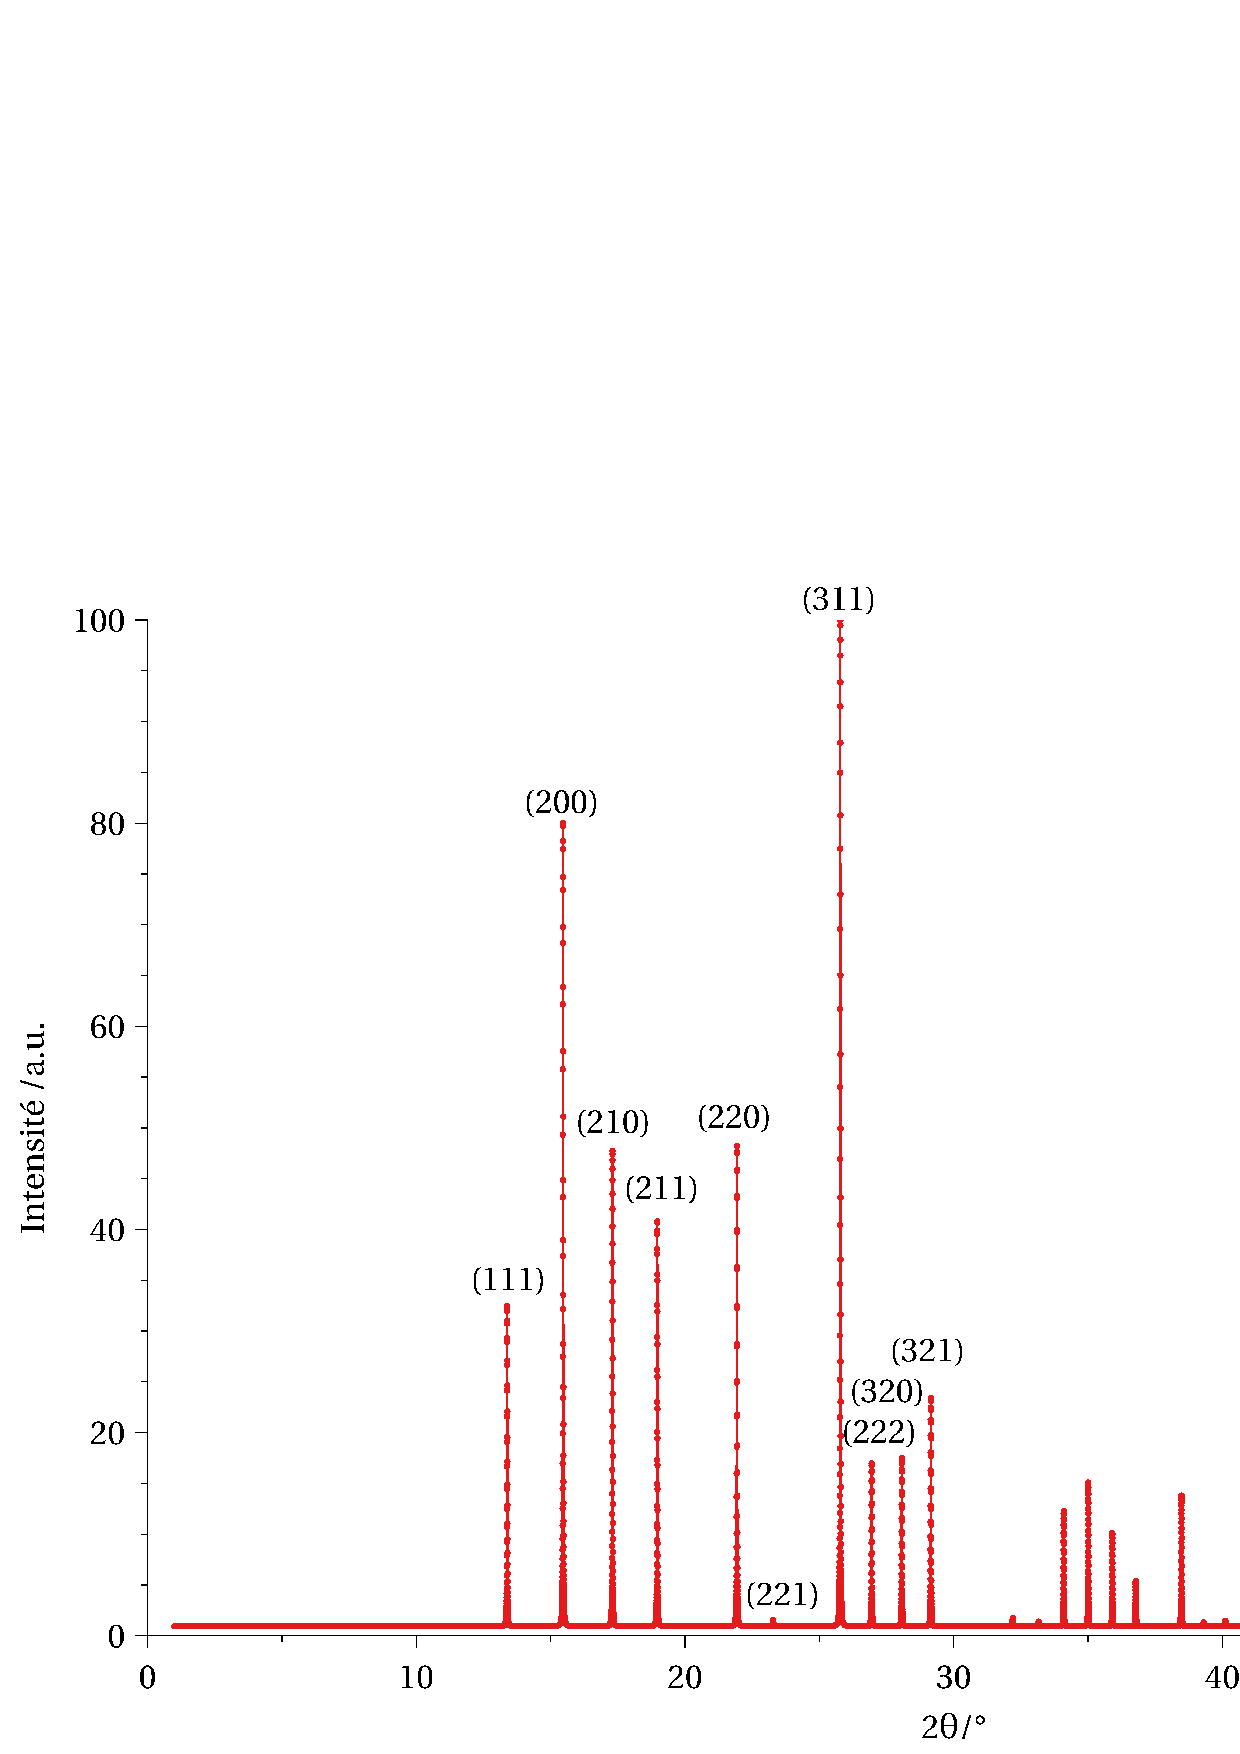
\includegraphics[width=\columnwidth]{figures/diffractogramme_pyrite.pdf}
\label{fig:soleilPowderDiffractogram}
\end{figure}

\begin{table*}[!tb]
\caption{Paramètres mesurés et calculés des 10 premières raies du diffractogramme de la \figref{fig:soleilPowderDiffractogram}.}
\label{tab:peaksParameters}
\centering
\begin{tabular}
  {
    c
    S[table-format = 2.3(1)]
    S[table-format = 1.4(1)]
    S[table-format = 1.4(1)]
    c
    c
    S[table-format = 1.4(1)]
  }      % Alignment for each cell: l=left, c=center, r=right
\toprule
\No de raie & % Numéro de raie
\ensuremath{2 \theta / \si{\degree}} & % 2*theta /°
\ensuremath{d_{hkl} / \si{\nano\metre}} & % d_hkl /nm
\ensuremath{\frac{d_{hkl,i+1}}{d_{hkl,i}}} & % d_(i+1)/d_i
\hmn{(hkl)} & % (hkl)
\ensuremath{h^2 + k^2 + l^2} & % h² + k² + l²
\ensuremath{a / \si{\nano\metre}}\\ % a /nm
\midrule
 1    & 13.38 & 0.3127 & 0.8867 & 111 & 3 & 0.5416 \cr
 2    & 15.45 & 0.2710 & 0.8938 & 200 & 4 & 0.5420 \cr
 3    & 17.30 & 0.2422 & 0.9131 & 210 & 5 & 0.5416 \cr
 4    & 18.96 & 0.2212 & 0.8663 & 211 & 6 & 0.5417 \cr
 5    & 21.92 & 0.1916 & 0.9427 & 220 & 8 & 0.5419 \cr
 6    & 23.27 & 0.1806 & {\cellcolor{red!25}}0.9044 & 221 & 9 & 0.5418 \cr
 7    & 25.77 & 0.1633 & 0.9573 & 311 & 11 & 0.5418 \cr
 8    & 26.94 & 0.1564 & 0.9608 & 222 & 12 & 0.5417 \cr
 9    & 28.06 & 0.1502 & 0.9637 & 320 & 13 & 0.5417 \cr
 10   & 29.14 & 0.1448 & {-}      & 321 & 14 & 0.5418 \cr
\bottomrule
\end{tabular}
\end{table*}\fxnote{Activer caption, sur un tableau multicolonnes et centrer valeurs SI}

On se contente d'utiliser les positions des 10 premières raies visibles sur le diffractogramme pour extraire les paramètres qui nous intéressent, et on numérote ces positions de 1 à 10.\\
À partir de ces valeurs d'angle \(2\theta\), on applique la loi de Bragg afin de retrouver les distances inter-réticulaires \(d_{hkl}\) associées à chacun des pics~:
\begin{equation}
n \lambda = 2 d_{hkl} \sin\theta,
\label{eq:BraggsLaw}
\end{equation}
avec \(\lambda = \lambda_{i,s} = \SI{0.07285}{\nano\metre}\), la longueur d'onde du faisceau incident utilisée, et \(n = 1\) en considérant uniquement des réflexions du premier ordre.

Chaque distance-inter-réticulaire est associée à une famille de plans donnée \hmn{(hkl)}.
On rappelle également que les distances inter-réticulaires dans le cas d'un réseau cubique obéissent à la formule~:
\begin{equation}
d_{hkl} = \frac{a}{\sqrt{h^2 + k^2 + l^2}},
\label{eq:dhklVsA}
\end{equation}
où \(a\) est le paramètre de la maille cubique et \(h\), \(k\) et \(l\) sont les indices de Miller associés aux plans dont on calcule l'espacement.\\
On remarque que des rapports de valeurs successives de ces distances inter-réticulaires peuvent être calculées de manière théorique en faisant varier les indices \(h\), \(k\) et \(l\) et pour chacun des modes de réseau d'une maille cubique (primitif \hmn{P}, centré \hmn{I} ou à faces centrées \hmn{F}).\\
Ces rapports correspondent simplement à des rapports de valeurs de \(\sqrt{h^2 + k^2 + l^2}\)~:
\begin{equation}
\frac{d_{hkl,i+1}}{d_{hkl,i}} = \frac{\left(\sqrt{h^2 + k^2 + l^2}\right)_{pic\, i}}{\left(\sqrt{h^2 + k^2 + l^2}\right)_{pic\, i+1}}.
\end{equation}
À condition de ne pas avoir d'extinctions dues au motif dans le diffractogramme expérimental, on doit pouvoir retrouver à quel mode de réseau appartient le cristal étudié, en comparant les rapports obtenus expérimentalement et les valeurs théoriques pour chacun des modes de réseau.\\
En effet, selon le mode de réseau, des extinctions typiques liées à une certaine parité des indices de Miller peuvent être prédites à partir du facteur de structure~: aucune extinction liée au réseau dans le cas d'un réseau \hmn{P}, des extinctions systématiques pour tous les \(h + k + l\) impairs dans le cas d'un réseau \hmn{I} et pour tous les \(h\), \(k\) et \(l\) de parité différente dans le cas d'un réseau \hmn{F}.\\
Ici, on trouve une correspondance avec les rapports caractéristiques d'un réseau cubique primitif (\hmn{cP}) puisqu'il y a moins d'extinctions que ne l'imposerait un autre mode de réseau.

\section{Calcul du paramètre de maille cubique}
% Remarque sur le rapport à valeur étrange et explication sur la raie manquante => obtention du d_hkl manquant
% Détermination du paramètre de maille cubique à partir des d_hkl (formule)
% Moyenne et écart-type de a

Afin de pouvoir estimer une valeur relativement précise du paramètre de maille \(a\), il faut déterminer les indices de Miller pour chacune des raies.\\
Pour la majeure partie, on se contente de se référer aux tables pré-calculées des rapports \(\frac{d_{hkl,i+1}}{d_{hkl,i}}\)~: pour chacun de ces rapports, on utilise les indices du \(i\)-ème \(d_{hkl}\), sauf pour le dernier pour lequel on est obligé d'utiliser le \(d_{hkl,i+1}\).

Il faut toutefois noter l'absence des raies associées aux familles de plans \hmn{(100)} et \hmn{(110)}.\\
De plus, lors de la comparaison des rapports de distances inter-réticulaires mesurées avec les valeurs théoriques, on a constaté que la valeur que l'on a associé à la raie \no 6, de très faible intensité, ne correspond à aucune valeur attendue.
Plus encore, il manque deux valeurs différentes impliquant trois raies (et trois rapports) en tout~: \(\frac{d_{310}}{d_{221}}\), \(\frac{d_{310}}{d_{300}}\) et \(\frac{d_{311}}{d_{310}}\).
Ceci est simplement la traduction d'une extinction due au terme de motif du facteur de structure.
Étant donné le fait que la seule combinaison en commun ici soit \hmn{310} et que les valeurs de \(d_{221}\) et \(d_{300}\) soient impliquées dans le calcul du rapport précédent avec la raie \no 5, on en déduit que la raie manquante est celle correspondant aux plans \hmn{(310)}.
Par conséquent, les indices à associer à la raie \no 6 sont, \textit{a priori} ceux des familles de plan \(d_{221}\) et/ou \(d_{300}\).

Pour le calcul des valeurs de a, on utilise l'\eqref{eq:dhklVsA}.\\
À partir de ces 10 valeurs calculées de a, on calcule une moyenne et l'écart-type de l'estimation obtenue~:
\begin{flalign}
a_{av} &= \SI{0.5417 \pm 0.000130}{\nano\metre} \\
       &= \SI{541.7 \pm 0.130}{\pico\metre} \nonumber
\end{flalign}

\section{Détermination du groupe d'espace}
% Directions manquantes sur le diffractogramme : 100, 110, 310
% Parité des directions manquantes et comparaison avec les IToC (annexe 3)
% Déduction du groupe d'espace
% Rasion de la faible intensité de la raie : 300 + 221 (extinction systématique de la 300)
% Explication extinctions élément de symétrie (élément translatoire => facteur de structure)

Comme remarqué précédemment, les raies associées aux familles de plans réticulaires \hmn{(100)}, \hmn{(110)} et \hmn{(310)} sont absentes du diffractogramme et ces extinctions ont été identifiées comme étant dues au terme de motif du facteur de forme.

On se réfère à la Table 3.1.4.1 des Tables Internationales de Cristallographie, \textit{Volume A} \cite{LooijengaVosIUCr2006} afin d'identifier le groupe d'espace exact à partir des conditions de réflexion.\\
Le groupe ponctuel et le mode de réseau étant connus pour être respectivement \hmn{m-3} et \hmn{P}, on restreint les possibilités aux seuls groupes d'espace \hmn{Pm-3}, \hmn{Pa-3} et \hmn{Pn-3}.
On peut aussi procéder à l'élimination immédiate du groupe \hmn{Pm-3} puisque celui-ci n'entraîne aucune extinction systématique alors que l'on sait qu'il y en a.\\
Enfin, on s'intéresse à la parité des raies éteintes pour le diffractogramme de la pyrite.
La différence entre \hmn{Pa-3} et \hmn{Pn-3} réside dans les conditions de réflexion pour des familles de plans d'indices \hmn{(0kl)} (les indices sont permutables de manière cyclique pour \hmn{Pa-3} et quelconque pour \hmn{Pn-3}).
Le groupe \hmn{Pn-3} comporte des réflexions pour tous \(k + l\) pairs dans le cas où \(h\) est nul.
Par permutation d'indices, on remarque que cette condition imposerait la présence de raies de diffraction d'indices \hmn{(110)} et \hmn{(310)}.
Puisque ce n'est pas le cas, on en déduit qu'il ne s'agit pas du bon groupe d'espace mais que la pyrite appartient au groupe \hmn{Pa-3}.
Le \(a\) qui vient remplacer le \(m\) dans la notation du groupe ponctuel correspond à l'introduction d'un élément de symétrie translatoire de type miroir avec glissement axial (forcément parallèle au vecteur \(\vec{a}\) du réseau de Bravais, dans un réseau cubique primitif).\\
Ceci est confirmé par le fait que la condition de réflexion de ce groupe pour les mêmes conditions que précédemment, avec \hmn{(0kl)}, est que seul \(k\) soit pair.
Par permutation cyclique pour retrouver les raies identifiées comme éteintes \hmn{(110)} et \hmn{(310)}, la condition pour une réflexion est que \(h\) soit pair.
Puisque sur ces deux raies \(h\) est impair, il est donc normal qu'une extinction survienne.

Par ailleurs, les conditions de réflexion pour des configurations avec un seul indice non nul \hmn{00l} sont synonymes d'un \(l\) pair (quelles que soient les permutations, cycliques ou non).\\
Ceci explique non seulement l'extinction constatée de la raie \hmn{(100)} mais également la faible intensité de la 6e raie du diffractogramme, censée comporter les contributions des familles de plans \hmn{(221)} et \hmn{(300)}.
Dans la pratique, on ne voit qu'une faible contribution des plans \hmn{(221)}.

\section{Positions atomiques}
% Positions atomiques (motif), sites de Wyckoff, ...
% Modèle VESTA
% Comparaison diagramme poudres VESTA vs expérimental SOLEIL
% Affinement par la méthode de Rietveld, vs. par tatonnement


Les derniers paramètres nécessaires à décrire complètement la structure de la pyrite (\ce{FeS2}) sont les positions atomiques au sein de la maille.

On commence par repérér la liste des sites de Wyckoff indiqués sur la fiche du groupe d'espace \hmn{Pa-3} (groupe \no 205) des Tables Internationales de Cristallographie, \textit{Volume A} \cite{IToCIUCr2016}, également accessibles sur le serveur de cristallographie de Bilbao \cite{BilbaoServer, Bilbao1,Bilbao2}.\\
Les premiers types de sites \(a\) et \(b\) de plus haute symétrie sont de multiplicité 4 et sont de même symétrie.
La deuxième plus basse multiplicité correspond aux sites \(c\) est 8, soit le double des sites \(a\) et \(b\) ce qui permet de faire coincider 4 unités formulaires de \ce{FeS2} avec les atomes de fer sur les premiers types de sites (on propose les sites \(a\)) et les atomes de soufre sur les sites \(c\).

De toutes les analyses précédentes notamment sur le groupe d'espace et les positions atomiques, on en déduit le facteur de structure associé à la pyrite~:
\begin{flalign}
F_{hkl} &= F_{\ce{Fe}} + F_{\ce{S}} &\\
        &= f_{\ce{Fe}} \left(\sum_j e^{-2\imath\pi(hx_j + ky_j + lz_j)}\right) \nonumber&\\
        &\quad + f_{\ce{S}} \left( \sum_j e^{-2\imath\pi(hx_j + ky_j + lz_j)}\right) \nonumber.&
\end{flalign}
où \(F_{\ce{Fe}}\) et \(F_{\ce{S}}\) correspondent aux facteurs de structure tenant compte de la liste des positions respectives de chacun des atomes de Fer et de Soufre.

À partir des coordonnées des sites de Wyckoff occupés et du groupe d'espace on est également en mesure de créer un modèle numérique de la maille élémentaire de la pyrite, comme celui de la \figref{fig:VestaModel}, à condition de faire une supposition sur les positions des atomes de Soufre dans la maille puisque seules des positions dépendant d'un offset \(x\) sont précisées comme coordonnées dans les Tables Internationales.
On fait la supposition initiale que ces atomes sont situés au centre des tétraèdres formés par les atomes de Fer (\(x = 1/4\)).\\
À partir de ce modèle il est également possible de générer un diagramme théorique de diffraction de poudre à comparer avec le diagramme expérimental obtenu sur synchrotron.
On se rend aisément compte du fait que les positions choisies arbitrairement pour les atomes de Soufre introduisent une symétrie plus grande que ne devrait fournir réellement le groupe d'espace, ce qui se traduit par un plus grand nombre d'extinctions que dans la réalité.
Il s'avère donc nécessaire d'affiner les paramètres de la structure pour retrouver les positions exactes des atomes de Soufre dans la maille.

Une première méthode, probablement la plus simple pour le faible nombre de paramètres présents ici (seule l'inconnue sur la valeur de \(c\) manque), consiste en une méthode par tâtonnements (ou \textit{trial and error})~: on ajuste la valeur de x manuellement jusqu'à arriver à un diffractogramme suffisament ressemblant à la version obtenur expérimentalement.\\
Une autre méthode plus précise et plus efficace peut être la méthode de Rietveld. Il s'agit d'une méthode numérique qui consiste à simuler successivement des diffractogrammes en les comparant à un diffractogramme expérimental (d'où la nécessité d'une mesure de bonne qualité), et en ajustant à chaque étape différents paramètres dont les positions atomiques qui influent directement sur le facteur de structure.
De manière générale, l'intensité des raies est proportionnelle au carré du module du facteur de structure~:
\begin{equation}
I_{hkl} \propto \left| F_{hkl} \right|^2,
\end{equation}
si bien que l'on peut obtenir une mesure de la qualité de l'affinement par comparaison avec l'intensité des raies expérimentales.\fxnote{Add refinement quality factor}
Il s'agit alors simplement d'appliquer une méthode des moindres carrés pour minimiser l'erreur entre théorie et mesure.\\
En plus du simple facteur de structure et des positions atomiques, d'autres paramètres liés à la polarisation incidente (facteur de Lorentz), à l'agitation thermique (facteur de Debye-Waller), à l'absorption, à la forme et à la largeur des raies doivent être ajoutés selon la configuration de l'expérience et le degré de précision désiré \cite{AlbinatiIUCr2006}.

\begin{figure}
\caption{Modèle de structure de la pyrite, réalisé avec le logiciel VESTA. Les positions atomiques sont les positions réelles après affinement de la structure}
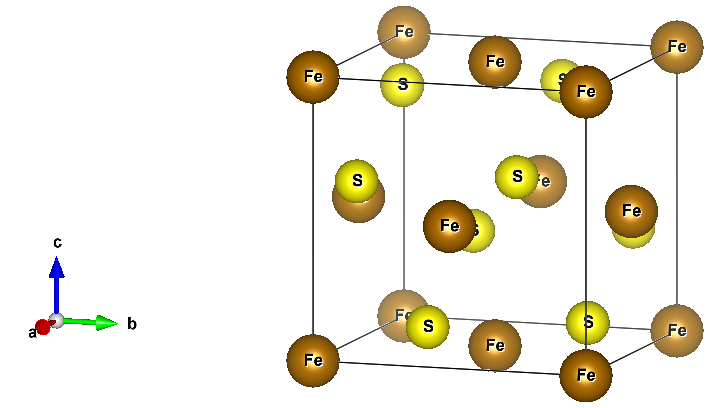
\includegraphics[width=\columnwidth]{figures/model_VESTA_FeS2}
\label{fig:VestaModel}
\end{figure}

On se contente ici de procéder par tâtonnements, ce qui permet de trouver une valeur pour \(x\) d'environ \num{0.38}.\\
Les atomes 
% Ajouter tableaux positions

\section{Conclusion}

% Conclusion et perspectives

